% Issue #76; owner: MilindDevX. Input from reports/phase2/main.tex.
% Numbers: results/metrics/fd001_interpretability_*.csv and the outputs of
% notebooks/phase2/14_interpretability.ipynb (#73). Figures:
% results/figures/fd001_interpretability_{ig,attention_gate}.png.

\section{Interpretability}
\label{sec:interpretability}

This section asks what the sequence models use to predict RUL, and whether
it matches what the Phase~1 tree models used. Every attribution explains the
frozen models of Section~\ref{sec:validation} on the 100 official FD001 test
engines, at each engine's last cycle, the cycle that was scored. No model is
retrained, and no test score changes.

\subsection{Method}
\paragraph{Integrated gradients}
For one input window, integrated gradients (IG)~\cite{Sundararajan2017axiomatic}
moves the input in a straight line from a baseline to the real window and
accumulates the model's gradients along the way. Each sensor at each of the
30 time steps then gets a share of the prediction, in cycles of RUL. The
baseline is the all-zero window, which puts every sensor at its training
mean because the inputs are z-scored on the training engines. The shares add
up to the prediction minus the baseline prediction. We check this
\emph{completeness} property, using 256 integration steps. The gap is at most
0.004 cycles for the Transformer and the LSTM. For the temporal CNN it is at
most 0.40 cycles, under 1\% of the roughly 45 cycles being attributed, because
its ReLU activations make the gradients less smooth. The Transformer, the best
sequence model in cross-validation, is the main subject. The LSTM and the
temporal CNN are analysed the same way, as a check on whether the findings
depend on the architecture. Every network is explained at all five seeds.

\paragraph{References and internal signals}
The sensor ranking is compared with SHAP~\cite{Lundberg2017unified}, the
attribution method used for the Phase~1 tree models. Engineered features are
credited to the sensor they come from. Two SHAP references are used. The
first is the Phase~1 ranking, from uncapped models explained on training
cycles. The second is the frozen XGBoost on engineered features, explained on
the same 100 test engines as the networks. We also read the Transformer's
attention weights and the gate of Hybrid~A on the test set.

\subsection{Results}

\begin{figure*}[t]
\centering
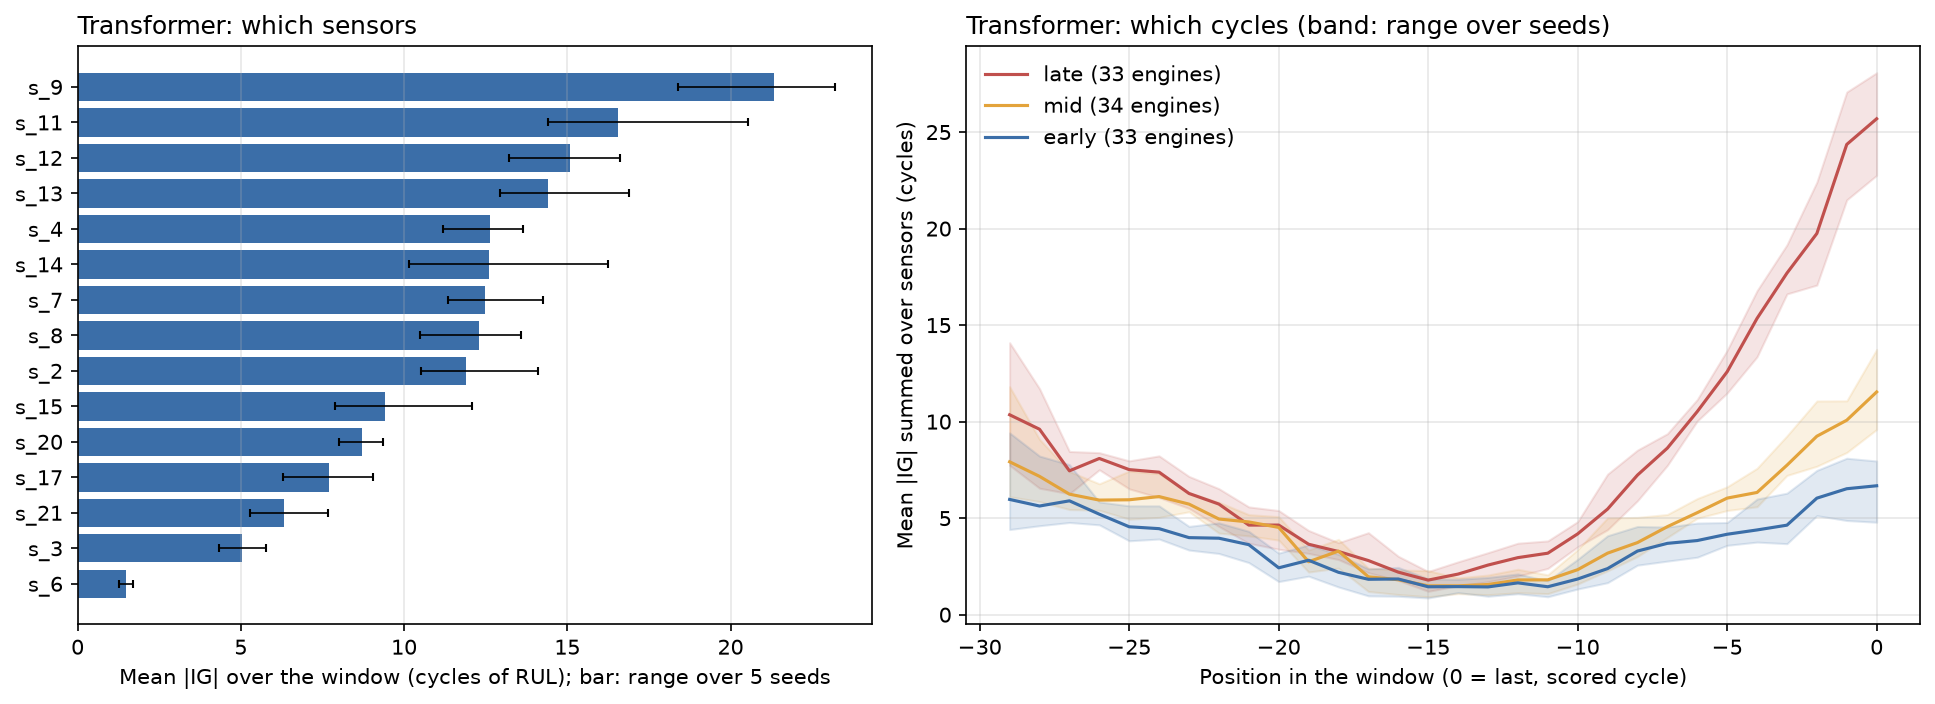
\includegraphics[width=\textwidth]{../../results/figures/fd001_interpretability_ig.png}
\caption{Integrated gradients for the Transformer on the 100 test engines.
Left: mean absolute attribution per sensor, summed over the window (bars:
range over five seeds). Right: mean absolute attribution per window position,
summed over sensors, by life stage. Position 0 is the last, scored cycle.}
\label{fig:interpretability_ig}
\end{figure*}

\paragraph{Which sensors}
The Transformer relies most on \texttt{s\_9}, then \texttt{s\_11},
\texttt{s\_12}, \texttt{s\_13} and \texttt{s\_4}
(Fig.~\ref{fig:interpretability_ig}, left). In the C-MAPSS
documentation~\cite{Saxena2008damage}, these are the physical core speed, the
static pressure at the high-pressure compressor outlet, the fuel-flow ratio,
the corrected fan speed and the low-pressure turbine outlet temperature.
\texttt{s\_6}, a bypass-duct pressure that is nearly constant on FD001,
contributes almost nothing. The ranking is stable: any two seeds agree with a
Spearman rank correlation of at least 0.86. The LSTM gives nearly the same
ranking (0.97, with the same top five sensors). The temporal CNN spreads its
attributions more evenly across sensors (0.74).

\paragraph{Agreement with SHAP}
Against SHAP for the XGBoost on the same test engines, the rank correlation
is 0.54, and three of the top five sensors are shared (\texttt{s\_9},
\texttt{s\_11}, \texttt{s\_4}). \texttt{s\_11} and \texttt{s\_4} rank near
the top in every SHAP ranking, including Phase~1's. The tree models give more
weight to \texttt{s\_15} and \texttt{s\_20}, and the networks to
\texttt{s\_12} and \texttt{s\_13}. Several C-MAPSS sensors move together as an
engine degrades, so two models can split credit between correlated sensors in
different ways while using the same information. The Phase~1 rankings agree
less (0.23 and 0.09). Those models were trained uncapped, their strongest
input was the cycle count itself (22 to 29 cycles of mean absolute SHAP), and
only their top 12 features were saved. With the cap, the XGBoost relies on
the cycle count far less (4.6). The sequence models never receive it, so their
predictions come from sensor behaviour alone.

\paragraph{Which cycles}
The attributions concentrate on the latest cycles of the window, and more so
near failure (Fig.~\ref{fig:interpretability_ig}, right). For engines in the
late stage, the Transformer puts 42\% of its attribution on the last 5 of 30
cycles, against 26\% for engines in the early stage (17\% would be uniform).
The LSTM and the temporal CNN show the same pattern more weakly. The
attributions also rise at the oldest cycles of the window, an edge effect we
did not investigate.

\begin{figure*}[t]
\centering
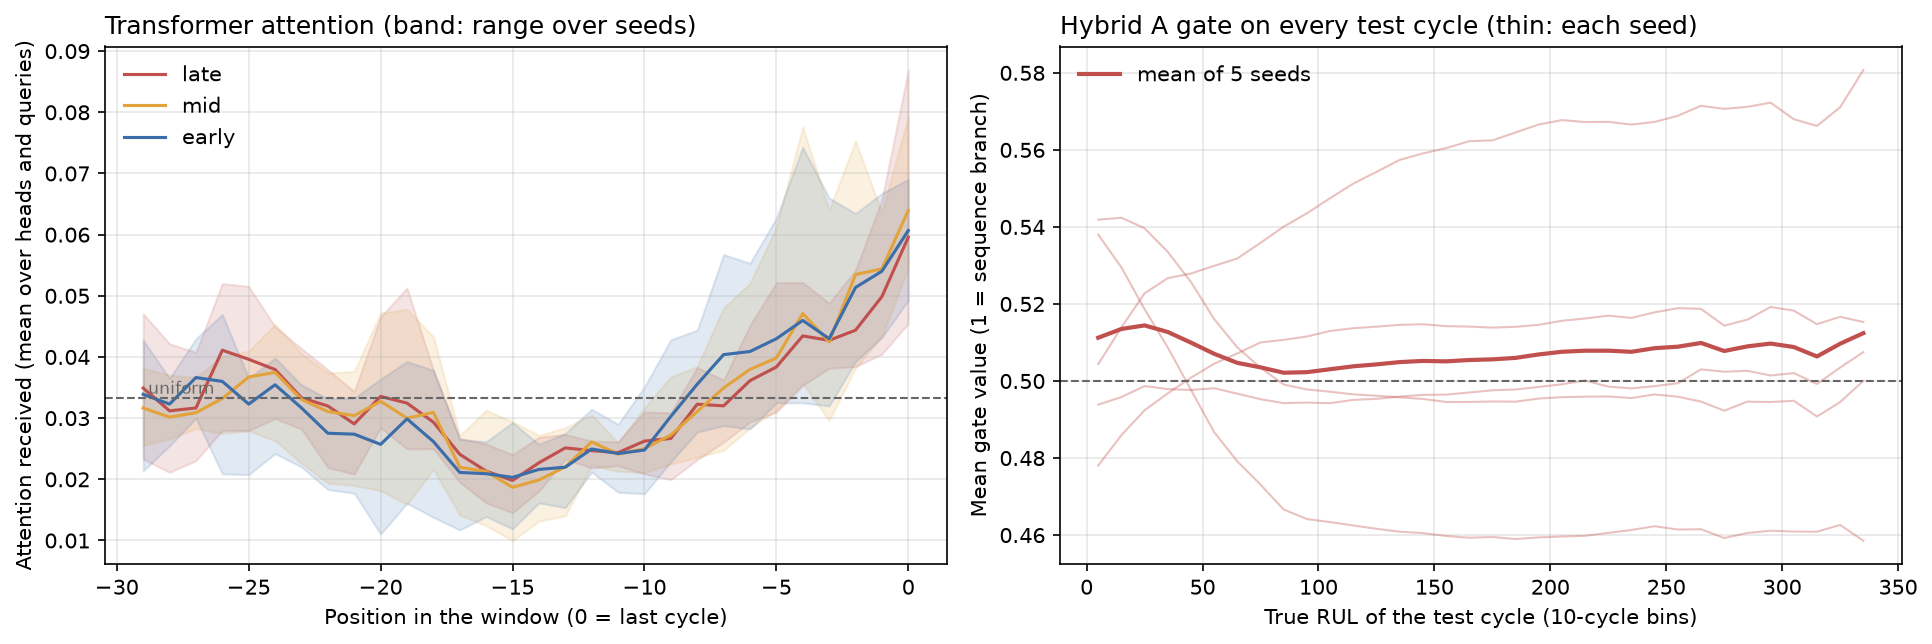
\includegraphics[width=\textwidth]{../../results/figures/fd001_interpretability_attention_gate.png}
\caption{Left: attention each window position receives in the Transformer,
averaged over heads, query positions, engines and seeds (band: range over
seeds); the dashed line is uniform attention. Right: the mean gate value of
Hybrid~A on every test cycle against its true RUL, for each seed (thin) and
their mean; 1 means the sequence branch.}
\label{fig:interpretability_attention_gate}
\end{figure*}

\paragraph{Attention and the gate}
The Transformer's attention does not show the shift seen in the attributions
(Fig.~\ref{fig:interpretability_attention_gate}, left). The last 5 cycles
receive 24--26\% of the attention at every stage. Attention weights describe
how information is mixed inside the model, not which inputs move its
prediction~\cite{Jain2019attention}, and here they are not a useful
explanation. Hybrid~A's gate stays close to 0.5
(Fig.~\ref{fig:interpretability_attention_gate}, right). By stage it ranges
from 0.46 to 0.56 over the five seeds, and its trend with the true RUL rises
for some seeds and falls for others. As in cross-validation, the gated
hybrid leans on neither branch on average, which matches its null result in
Section~\ref{sec:validation}.

\subsection{Limits}
Integrated gradients depend on the baseline, and a different reference window
would change the attributions. Absolute attributions measure how much an
input matters, not in which direction it moves the prediction. Correlated
sensors share credit arbitrarily, so a low rank does not mean a sensor carries
no information. The attributions describe what these fitted models compute on
100 test engines at their last cycle. They are not evidence of how an engine
degrades physically. Finally, the Phase~1 comparison covers only the 12
features that its notebook saved.
